\documentclass{llncs}

\usepackage{geometry}
\geometry{
  a4paper,         % or letterpaper
  textwidth=15.5cm,  % llncs has 12.2cm
  %textheight=24cm, % llncs has 19.3cm
  %heightrounded,   % integer number of lines
  hratio=1:1,      % horizontally centered
  %vratio=2:3,      % not vertically centered
}
\usepackage{makeidx}
\usepackage{amsmath}
\usepackage{graphicx}
\usepackage{indentfirst}
\usepackage{booktabs}
\usepackage{subfigure}
\usepackage{multirow}
\usepackage{changepage}
\usepackage{epsTopdf}
\setlength{\parindent}{1em}

\begin{document}
\frontmatter
\pagestyle{headings}

%\mainmatter

	\title{Joint User Attributes and Item Category in Factor Models for Rating Prediction}
%	\author{Jiang Wang$^{\dag}$, Yuqing Zhu$^{\ddag}$, Deying Li$^{\dag}$}
%	$^{\dag}$School of Information Renmin University of China, Beijing, China, Email: \{jiangw, deyingli\}@ruc.edu.cn}\\
%    $^{\ddag}$Department of Computer Science, California State University at Los Angeles, Los Angeles, CA, USA 90032,Email: %yzhu14@calstatela.edu     }

    \author{Jiang Wang$^{\dag}$, Yuqing Zhu$^{\ddag}$, Deying Li$^{\dag}$, Wenping Chen$^{\dag}$, Yongcai Wang$^{\dag}$}
    \institute{$^{\dag}$School of Information,  Renmin University of China, Beijing, China 100872\\
    $^{\ddag}$Department of Computer Science, California State University at Los Angeles, Los Angeles, CA, USA 90032\\
    \email{\{jiangw, deyingli, wenpingchen, ycw\}@ruc.edu.cn,yzhu14@calstatela.edu}}
	\maketitle
	\begin{abstract}
		\noindent One important problem of recommender system is rating prediction.
		In this paper, we use the movie rating data from MovieLens as an example to show how to use users' attributes to
		improve the accuracy of rating prediction.
		Through data analysis, we observe that users having similar attributes tend to share more similar preferences and
		users with a special attribute have their own preferred items.
		Based on the two observations, we assume that a user's rating to an item is determined by both the user intrinsic characteristics and the user
		common characteristics. Using the widely adopted latent factor model for rating prediction,
		in our proposed solution, we use two kinds of latent factors to model a user: one for the user intrinsic characteristics and the
		other for the user common characteristics. The latter encodes the influence of users' attributes which include user age, gender and occupation.
		On the other hand, we jointly use user attributes or item category information and rating data for calculating similarity of users or items.
		The similarity calculating results are used in our proposed latent factor model as a regularization term
		to regularize users or items latent factors gap.
		Experimental results on MovieLens show that by incorporating users' attributes influences,
		much lower prediction error is achieved than the state-of-the-art models.
		The prediction error is further reduced by incorporating influences from item category popularity and item popularity.
		
	\end{abstract}
%	
%	% A category with the (minimum) three required fields
%	%\category{\noindent H.3.3}{Information Search and Retrieval}{Information filtering;}
%	%A category including the fourth, optional field follows...
	
	
	\keywords{Recommendation; Rating prediction; Matrix factorization} % NOT required for Proceedings
	
	\section{INTRODUCTION}
	With the rapid increasing of web information, recommender system is becoming more and more popular since it is good for both consumers and service or product provider.
	On one hand, it helps consumers to alleviate the information overload problem. On the other hand, it brings better sales to product or service provider.
	Diversity recommender systems have been designed to meet the needs of different platforms in recent years.
	Such as commodities recommendation for E-commerce websites, friends recommendation for social network platform
	and point-of-interest recommendation for location-based social networks (LBSN).
	
	Depending on the application, different recommendation problems have been defined and studied.
	The top-N item recommendation and rating prediction are two most widely studied categories of recommendation problems.
	On one hand, top-N item recommendation tasks aim to recommend a user a list of items that she may be interested in.
	For example, in movie websites, movie recommendation aims to recommend unseen movies to users.
	Rating prediction, on the other hand, is to predict the preference rating of a user to a product or service that she has not rated before.
	The products or services with high predicted ratings are recommended to users. In this study, we are interested in
	the movie rating prediction problem with user attribute data from MovieLens.
	
	In recent years, social information is widely used in the recommendation system and the performance has been improved a lot.
	One popular method using social information in recommendation systems is SocialMF\cite{SIGIR201301}.
	SocialMF is proposed by adding the social regularization term to the matrix factorization objective function.
	The additional social regularization term ensures that the distance of the latent vectors of two users or items will become closer
	if  two users or items are more similar.
	Commonly, users' or items' similarity are computed based on user-item ratings,
	which is not applicable for new users or items.
	In our dataset, both user attributes and item categories information are available.
	For item rating prediction, an interesting question here is:
	Are the user attributes and item categories information helpful to similarity calculation
	and can they improve the accuracy of rating prediction?
	
	%In our study, the similarity of two users is a linear combination of rating similarity and attribute similarity,
	%which can partly to slow down cold start user problem and is more accurate than only using rating similarity.
	%On the other hand, we utilize items' category information for item similarity calculation to ensure higher accuracy.
	
	To answer the question above, we conducted data analysis on
	MovieLens's movie rating data. We observe that users having similar attributes tend to share more similar user
	preferences and users with certain attribute have their own favorite items, while other users without that attribute may not be interested in
	those items.
	Based on these observations, we incorporate user attributes influences into our movie rating prediction model which is based on
	the widely adopted latent factor model realized by Matrix Factorization (MF). Together with influences from other factors including
	item category, user neighbor, item neighbor, item popularity and item category popularity,
	we show that the proposed model outperforms state-of-the-art baselines including Biased MF, RSVD and Social MF\cite{SIGIR201301,4-1-1},
	measured by both Mean Absolute Error (MAE) and Root Mean Square Error (RMSE).
	To the best of our knowledge, this is the first study exploiting user attributes as latent factor in item rating
	prediction. To summarize, the main contributions arise from
	this study are as follows:
	
	\begin{adjustwidth}{0.5cm}{0cm}
		$\bullet$ We conduct data analysis and observe that users having similar attributes tend to share more similar user
		preferences and users with certain attribute have their own favorite items, while other users without that attribute may not be interested in
		those items. This is an important observation that
		could be useful for not only item rating prediction, but
		also related studies, e.g., item recommendation and user attribute
		analysis from rating data.
	\end{adjustwidth}
	\begin{adjustwidth}{0.5cm}{0cm}
		$\bullet$ We directly model the influence of user attributes into movie rating prediction using matrix factorization.
		Specifically, for each user, we use two different latent factors to represent his or her intrinsic and common characteristics respectively.
		Every user's intrinsic latent factors are unique and determined by himself or herself. While common latent factors of a user are determined by
		his or her attributes' type and every attribute has a latent factors.
		On the whole, a user's latent factors are modeled as the linear combination of his or her intrinsic latent factors and all attributes' latent factors.
		In our recommender system, we have also considered other factors including item popularity and item category popularity.
		To the best of our knowledge, this is the first
		study that models user attribute influence as latent factors into rating prediction, while previous studies only take a attribute as a bias.
	\end{adjustwidth}
	\begin{adjustwidth}{0.5cm}{0cm}
		$\bullet$ We conducted extensive experiments to evaluate the effectiveness of incorporating influence of user attributes and other factors in
		item rating prediction and compared the prediction accuracy of the proposed model with an
		array of strong baseline models. The experiment results show  that using both user or item profile information and rating sequence information
		for selecting appropriate neighbor can further improve the performance and different user attributes have imparity
		status in item rating prediction.
		
	\end{adjustwidth}
	
	
	
	The rest of this paper is organized as follows. We review the
	related work
	in Section 2. The data analysis is reported in Section 3.
	The details of the proposed item rating prediction model
	is presented in Section 4, Experimental evaluation is showed in Section 5.
	Finally, Section 6 concludes this paper.
	
\section{RELATED WORK}
	The collaborative filtering (CF) technique has become more and more popular in personalized recommender task\cite{2-1-1,2-1-2,2-1-3,2-1-4} since CF methods are domain independent and only require the past activities history of users,
	i.e. user-item rating matrix, to make recommendations.
	According to different means of utilizing the user-item
	rating matrix, collaborative filtering approaches are usually divided into two kinds of categories\cite{cfclass}: memory-based
	CF and model-based CF.
	
	Memory-based CF, also called as neighbor-based methods, use the history user rating behaviors data for recommendations.
	The basic idea of memory-based CF  is to find similar users or items for target user or item by using similarity measures.
	Once the neighborhoods are formed, memory-based CF usually takes a weighted sum of ratings given by their
	neighbors (target user' neighbors or target item' neighbors) as a prediction.
	user-based CF\cite{cfclass,uCF} and item-based CF\cite{iCF1,iCF2} are two typical kinds of  memory-based method.
	User-based CF predicts the ratings based on the opinions of target user's
	neighbors, which have similar item preferences with target user.
	On the other hand, item-based CF provide prediction based on the ratings of items that is similar to target item.
	
	In contrast with memory-based CF,
	which utilize entire user-item matrix to provide recommendations for target users,
	model-based CF make use of statistical and machine learning techniques to learn a predictive model from training
	data. The predictive model can characterize the rating
	behaviors of target users. Then model-based CF use the trained model to predict the unobserved ratings,
	rather than directly utilize the entire user-item matrix to compute predictions.
	Latent factor model is one of the most successful CF models, in which users and items are jointly
	mapped into a shared latent space of much lower dimensionality.
	As the most successful realization of latent factor model, matrix
	factorization (MF) \cite{SIGIR201301,KDD200801,COMPUTER2009} has been successfully applied to various recommender systems
	including location rating prediction for
	Jiepang \cite{GeoMF} and Yelp \cite{SIGIR201401}, event recommendation for Meetup\cite{event1}
	and Douban \cite{event2}, and personalized tweet tag recommendation \cite{tag}.
	
	Among various MF models proposed, SVD++ \cite{KDD200801} is probably
	one of the most successful models. This model integrates the implicit feedback information from a user to items (e.g., based on
	user' s purchase history or browsing history). More specifically, the
	user vector of latent factors in this model is complemented by the
	latent factors of the items to which the user has provided implicit
	feedback. Recently, Ma \cite{SIGIR201301} proposed a social regularization MF
	method, named Social MF, to employ the similar and dissimilar
	relationships between users and items to improve recommendation accuracy. The similarity between items is measured based on
	their ratings using Pearson' s correlation or cosine similarity.
	It is usually difficult to reflect the real similarity of two users or items that only using the rating information to measure similarity.
	In many literatures, many other user-/item-specific attributes are introduced to calculating user similarity or item similarity.
	In contrast with rating data, user attribute information, for example,
	age, gender, occupation for a user, can represent the characteristics more accurately.
	Item has a similar situation with user.
	In our experiments, user attribute information and item category information are introduced to calculating similarity,
	and the proposed models achieve better rating prediction
	accuracy than Social MF \cite{SIGIR201301} indicating that adding the influence from attributes neighborhood is more effective than the influence only from
	neighbors chosen by rating-based similarity measures.
	
	Based on MF, influence from other aspects of users or items besides the ratings can be flexibly and easily modeled. For example,
	Koenigstein et al. \cite{bias} incorporated rich item bias into MF model to
	capture the taxonomy information of music. Each music has multiple types of information such as track, album, artist and genre. In
	their proposed model, MF was extended by adding shared bias parameters for items linked by common taxonomy. Moreover, some
	other work has also shown that popularity is helpful in improving
	the recommendation accuracy \cite{popular1,popular2}.
	To the best of our knowledge, user or item attributes are introduced to most of literatures as biases.
	However, few work focus on taking user or item attributes information as latent factors to
	improve the quality of recommendation.
	In our problem setting, we consider the attributes from a user
	further elaborates about the rating. We model users' attributes
	as latent factors and incorporate the attributes into rating prediction.
	Next, we conduct data analysis of the MovieLens data.
	\section{DATA ANALYSIS}
	\subsection{Dataset}
	Our study is based on the popular released MovieLens Dataset\footnote{http://www.grouplens.org/system/files/ml-100k.zip.}.
	The data was collected through the MovieLens web site\footnote{movielens.umn.edu} during the seven-month period from September 19th,
	1997 through April 22nd, 1998. It contains 100,000 user-item ratings (scale from 1 to 5) rated by 943 users on 1,682 items.
	
	This data has been cleaned up \-- users who had less than 20 ratings or did not have complete demographic
	information were removed from this data set. A user contains a unique id, name, age, gender and occupation.
	This data have 21 occupations and a user only has one of them. An item has a unique id, name, release date, URL
	and its categories. This data have 19 categories and an item may have more than one category.
	However, we don't use released date and URL in our study. A rating tuple contains user id, item id, rating from 1 to 5 stars and date.
	In this study, we do not use the date feature for its less relevance to our research problem.
	Table 1 reports the minimum, maximum, and average number of ratings per user and per item respectively.
	\begin{table}\label{DataSet}
		\centering
		\caption{Statistics of Dataset MovieLens}
		\begin{tabular}{l|l|l} \hline
			Statistics& User &Item\\ \hline
			Min. Num. of Ratings& 20& 1 \\ \hline
			Max. Num. of Ratings& 737 &583\\ \hline
			Avg. Num. of Ratings& 106.04 &59.45\\ \hline
		\end{tabular}
	\end{table}
	\subsection{Observations}
	
	To gain a better understanding of users' rating behaviors, we
	study the rating data introduced above.
	More specifically, we study the influence of user attributes for rating behavior at two levels: item-level
	and rating-level. We make two observations from the data analysis: a) Users have similar attributes tend to share more similar user
	preferences; and b) Users with certain attribute have their own favorite items, while other users without that attribute may not be interested in
	those items. These patterns are independent of
	any particular user. We now report the details of the data analysis.
    \\
	
	\noindent\textbf{Item Level.} To better study users rating behaviors at rating level,
	we cluster the users into groups by user attributes. Users having same attribute value are
	clustered in same group. As an example, we cluster users into female group and male group by gender.
	In order to observe the item level rating behaviors more intuitively,
	we measure the Rating Count Difference(RCD) of each item $i$ for two user groups $us_j$ and $us_k$,
	these two user groups have different attribute value $a_j$ and $a_k$, respectively.
	Considering the user number gap of those two user groups, using Absolute Rating Count Difference(ARCD) is unfair.
	Hence we use Normalized Rating Count Difference(NRCD) to measure RCD, defined as follows.
	\begin{equation}
		NRCD_i(us_j, us_k) =\frac {\frac {\sum\limits_{t \in I} {\mid us_{kt}\mid}}{\sum\limits_{t \in I}{\mid us_{jt}\mid}}\cdot\mid us_{ji}\mid - \mid us_{ki}\mid} {\max\limits_{t \in I} ({{\frac {\sum\limits_{t \in I}{\mid us_{kt}\mid}}{\sum\limits_{t \in I}{\mid us_{jt}\mid}}\cdot\mid us_{ji}\mid - \mid us_{ki}\mid)}}}
	\end{equation}
	Where $NRCD_i(us_j, us_k)$ is normalized rating count difference of user group $us_j$ and user group $us_k$ for item $i$,
	I is the set of all items,
	$us_{ji}$ and $us_{ki}$  denote the two sets of users who have rated item $i$,
	and $\mid\bullet\mid$ denotes the cardinality of a set.
	
	\begin{figure*}
		\centering
		\begin{minipage}{0.48\linewidth}
			\centerline{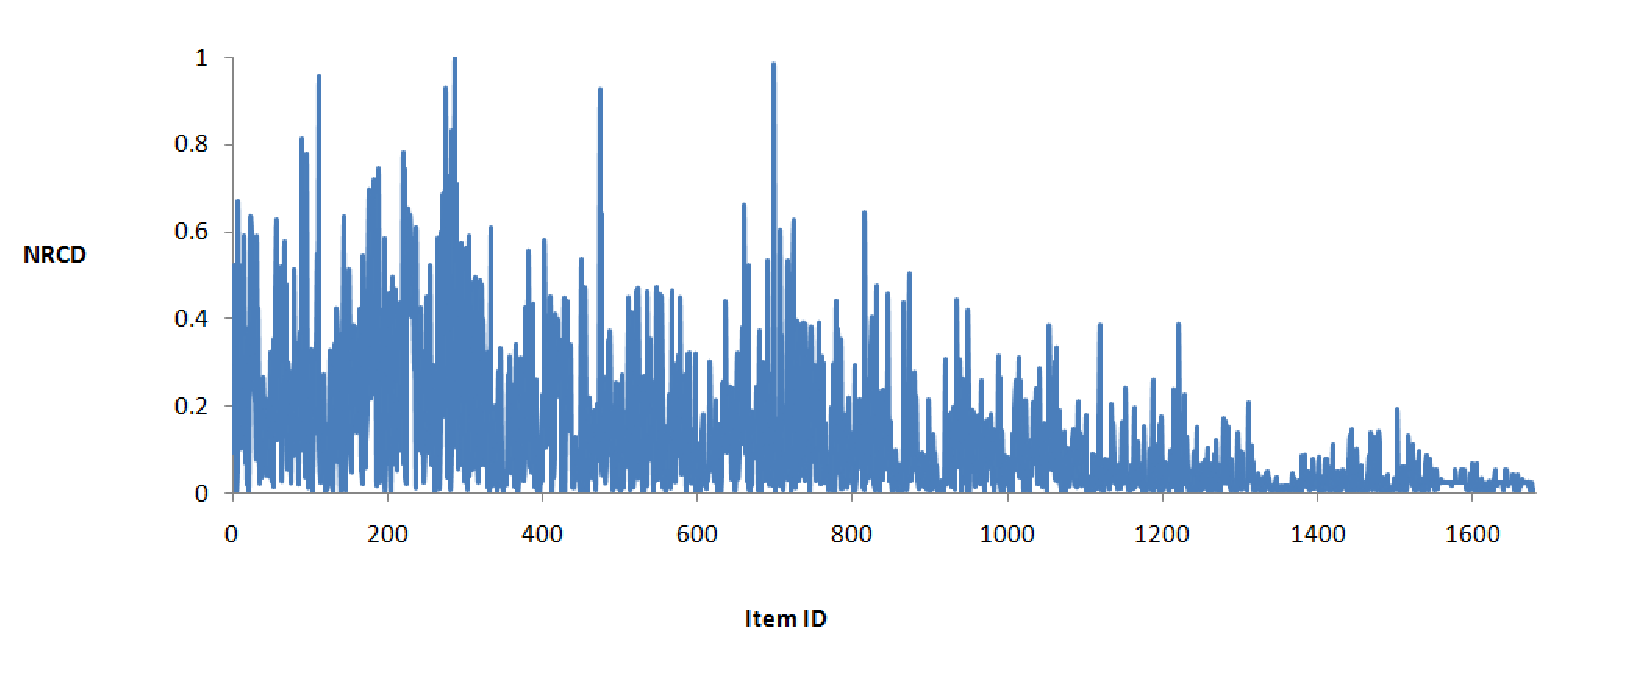
\includegraphics[height=4cm, width=12cm]{gender_female_male_RCD.eps}}
		\end{minipage}
		\caption{\textbf{Normalized Rating Count Difference(NRCD) of Female and Male }}
	\end{figure*}
	
	Figure 1 plots the rating count difference(NRCD) of female and male.
	As shown in Figure 1, female's rating count for each item shows great difference to male's. Specifically, about 13\% items' NRCD is over 0.3
	and average of NRCD is about 0.13. Another interesting phenomenon is about 45\% items' NRCD less than 0.05. These two phenomena indicate that female
	and male share similar preferences for most of items, while for some particular items, their preferences show huge gap.
	In other words, users' gender has a certain degree of influence for users' rating behaviors. For age (3 age groups )
	and occupation (21 occupations), Rating count difference have similar circumstance with gender. As a result of the limitation of space,
	we omit the NRCD figures of age groups and occupations. Table 2 lists top-5 ARCD items of young adults and mid adults.
	Item 286 has the max ARCD of 213, while the max NRCD of items is 515. This is because NRCD and ARCD are two measure methods which have
	a certain relation, but inequitable. Any way, these two measure methods both
	indicate user attributes have influence of user's rating behaviors in another way.
	\begin{table}
		\centering
		\caption{Top-5 ARCD Items of Young Adults(YA) and Mid Adults(MA)}
		\begin{tabular}{c|c|c|c|c} \hline
			Item ID &RC YA &RC MA &NRCD & ARCD \\ \hline \hline
			286	&87	&300	&0.67	&\textbf{213}\\ \hline
			269	&54	&206	&0.55	&152\\ \hline
			515	&13	&151	&\textbf{0.83}	&138\\ \hline
			211	&19	&152	&0.74   &133\\ \hline
			483	&37	&169	&0.57	&132\\ \hline
		\end{tabular}
	\end{table}
	\\
	\noindent\textbf{Rating Level.} At the rating level, we analyze the
	average of each item's rating for diverse user groups.
	Without loss of generality, we use student group and educator group as an example.
	These two user groups clustered according occupation.
	To avoid the influence of sparse data,
	we don't consider items which are less than 5 user rated in either student or educator.
	After the preprocessing, only 500 items remind. But we surprising discover that about 30\% items'
	average difference are larger than 0.5. Especially, the max gap reaches 1.46 for item 919.
	More detailed statistics of these two groups are summarized in Table 3.
	\begin{table}
		\centering
		\caption{Statistics of Student(S) and Educator(E)}
		\begin{tabular}{c|c|c|c} \hline
			Statistics & Item id & Group& Diff  \\ \hline \hline
			Max. of Avg Ratings Difference &919 &- &1.46 \\ \hline
			Min. of Avg Ratings Difference &257,etc. &- &0 \\ \hline
			Avg. of Avg Ratings Difference &- &- &0.32 \\ \hline
			Max. of Avg Ratings  &170 & S &4.93 \\ \hline
			Max. of Avg Ratings  &48 & E &4.69 \\ \hline
		\end{tabular}
	\end{table}
	
	We also compare others user group pairs, they have similar circumstance with student and educator group.
	From these analysis in rating level, we can get a similar conclusion with item level --- user attributes
	have certain influence for user rating behaviors.
	
	Motivated by the two observations, we propose incorporating the
	above attribute characteristics for rating prediction, so as to improve item recommendation accuracy.
	
\section{RATING PREDICTION}

    Rating prediction is a basic problem in recommendation system and  has been widely studied in literature.
    In this paper, we use $r_{ui}$ to denote the rating that user $u$ gives to item $i$ (i.e., a movie),  and
    $r_{ui}$ is in the range of $1$ to $5$ stars with more stars indicating higher preference.
    Given the existing ratings made by $M$ users to $N$ items, the task is to predict the unknown rating $\hat{r}_{ui}$,
    if user $u$ has not rated item $i$ before. In the following, we first briefly
	introduce matrix factorization and then present our proposed model
	by incorporating various influences into the prediction. Table 4 lists
	the notations used in this paper.
	\begin{table}
		\centering
		\caption{Notations and semantics}
		\begin{tabular}{l|l} \hline
			$N_i$&Set of neighbors of item $i$\\
			$K$ & Set of ($u$,$i$) pairs with known $r_{ui}$ ratings\\
			$T$ & Set of ($u$,$i$) pairs using test\\\hline
			$s_{uf}$ & Similarity of user(item) $u$ and user(item)$f$ \\
			$s^a_{uf}$ & Attribute similarity of user(item) $u$ and user(item)$f$ \\
			$s^r_{uf}$ & Rating similarity of user(item) $u$ and user(item)$f$ \\
			$r_{ui}$ & Observed ratings of user $u$ to item $i$\\
			$\hat{r}_{ui}$ & Predicted ratings of user $u$ to item $i$\\
			$\mu$& Mean of all known $r_{ui}$ ratings \\
			$b_u$ & Bias parameters for user $u$  \\
			$b_i$ & Bias parameters for item $i$ \\ \hline
			$\mathbf{p}_u$& Latent factors of user $u$\\
			$\mathbf{q}_i$& Latent factors of item $i$\\
			$\mathbf{a}_{ua}$& Latent factors of user $u$'s age group\\
			$\mathbf{g}_{ug}$& Latent factors of user $u$'s gender \\
			$\mathbf{o}_{uo}$& Latent factors of user $u$'s occupation \\\hline
			$\gamma$ &Similarity weighting parameter \\
			$\rho_i$ & Normalized popularity of item $i$ \\
			$\gamma_i$ &Popularity weighting parameter for item $i$\\
			$\tau_c$ & Normalized popularity of item category $c$\\
			$\gamma_c$ & Popularity weighting parameter for item category $c$\\ \hline
		\end{tabular}
	\end{table}
	\subsection{Matrix Factorization}
    Our proposed method is based on the latent factor model realized
	by matrix factorization. Matrix factorization map users and items into a
    joint latent space with dimension $f << min(M; N)$.
    The inner product of a user vector $\mathbf{p}_u\in R^{f\times1}$
	and an item vector $\mathbf{q}_i\in R^{f\times1}$ is used to approximate the user's
	preference to the item (see \cite{4-1-2} for a detailed introduction of matrix
	factorization). Accordingly, the predicted rating of user $u$ to item $i$
	is computed using

	\begin{equation}\label{1}
		\hat{r}_{ui}=\mathbf{p}_u^T\mathbf{q}_i,
	\end{equation}
	where $\mathbf{p}_u$ and $\mathbf{q}_i$ can be learned from the user-item rating matrix
	with known ratings. However, users may have certain degree of biases:
	some users are more lenient and some are very strict about ratings.
	Similarly, items may also have some degree of biases because of location or branding for example.
	To achieve more accurate rating prediction, Biased MF extends the basic matrix factorization by
	considering the biases,
	\begin{equation}\label{2}
		\hat{r}_{ui}=\mu+b_u+b_i+\mathbf{p}_u^T\mathbf{q}_i,
	\end{equation}
	where $\mu$ is the average rating of all known ratings, $b_u$
	and $b_i$ are the user bias and item bias, respectively.
	Learning the unknown parameters $\mathbf{p}_u$, $\mathbf{q}_i$, $b_u$ and $b_i$ is
	an optimization problem to minimize the regularized squared error on
	the set of known ratings $K$ .
	\begin{eqnarray*}
		\min_{p^\star,q^\star,b^\star} &\sum_{(u,i)\in K} {(r_{ui}-\hat{r}_{ui})^2}+
		\lambda_1(\parallel{\mathbf{p}_u}\parallel^2+\parallel{\mathbf{q}_i}\parallel^2)
		&+\lambda_2(b_u^2+b_i^2)
	\end{eqnarray*}
    In this equation, $\lambda_1$ and $\lambda_2$ are regularization parameters used to avoid overfitting.
	Both stochastic gradient descent (SGD) and alternating least squares (ALS) algorithms
	can be used to solve the optimization function and learn the parameters \cite{4-1-1,4-1-2}.
	In this paper, we adopt SGD to learn the parameters following the algorithm
	presented in \cite{4-1-1}.
	
\subsection{Incorporating Neighborhood Influence}
	Inspired by \cite{SIGIR201301,4-2-1}, user or item neighbors information can help rating prediction.
	In the case of missing explicit neighbor information in MovieLens, we
	use top-N similar users of target user instead of his or her neighbors information and
	then plug in those similar users to the aforementioned matrix factorization framework.
	There are several methods we can borrow in the literature
	to compare the similarity between two users. In this paper,
	we jointly adopt rating similarity and attribute similarity, which is defined as:
	
\begin{eqnarray*}
		&&s_{uf}=\gamma\cdot s^a_{uf}+(1-\gamma)\cdot s^r_{uf} \\
        &&s^r_{uf} = \frac {\sum_{k \in I(u)\cap I(f)}(r_{uk} - \bar{r}_u)\cdot(r_{fk}-\bar{r}_f)} {\sqrt{\sum_{k \in I(u)\cap I(f)}(r_{uk} - \bar{r}_u)^2} \cdot \sqrt{\sum_{k \in I(u)\cap I(f)}(r_{fk} - \bar{r}_f)^2} }\\
        &&s^a_{uf} = \frac {1}{3} (s^{age}_{uf} + s^{gender}_{uf} + s^{occupation}_{uf})
	\end{eqnarray*}
	
\noindent where $s_{uf}$ is the similarity between user $u$ and $f$, $s^r_{uf}$ indicates the
	rating similarity and we adopt Pearson Correlation Coefficient(PCC) to calculate it.
$I(u)$ is a set of items that rated by user u, and $\bar{r}_u$ represents the average rate of user u.
$s^a_{uf}$ represents the attribute similarity and it's a linear combination of age, gender and occupation similarity.
    Age similarity $s^{age}_{uf}$ is a normalized value of the age difference of user $u$ and $f$.
    Gender similarity $s^{gender}_{uf}$ is equal to 1 if the gender of user $u$ and $f$ are the same, otherwise it is a small smooth value.
    The calculation method of occupation similarity $s^{occupation}_{uf}$ is similar to $s^{age}_{uf}$.
	And parameter $\gamma$ is introduced to balance the importance between rating and attribute similarity.
	Incorporating neighborhood influence, we proposed the matrix factorization objective function as follow:
	
\begin{eqnarray*}
		\min_{p^\star,q^\star,b^\star} &&\sum_{(u,i)\in K} {(r_{ui}-\hat{r}_{ui})^2}+
		\beta_1\sum_{f \in N(u)}s_{uf}\parallel{\mathbf{p}_u-\mathbf{p}_f}\parallel^2 +\lambda_1(\parallel{\mathbf{p}_u}\parallel^2
        +\parallel{\mathbf{q}_i}\parallel^2) \\
        &&+\lambda_2(b_u^2+b_i^2)
	\end{eqnarray*}
	
\noindent where $\beta_1$ is the regularization parameter,
	and $N(u)$ represents user $i$'s neighbors.
	In this method, the neighbors information is employed in designing the neighbor regularization term to constrain the matrix factorization objective function. The neighbor regularization term also indirectly models the difference
	of users' tastes. More specifically, if user $u$ has a high similarity with  user
	$f$, this regularization term actually indirectly minimizes the distance between latent vectors $\mathbf{p}_u$ and
	$\mathbf{p}_f$.
	
	From the above, since we define the implicit user social information as the similar users, we can naturally
	extend this idea to take advantages of the implicit item
	social information, which can be found through the similar items.
    The similarity calculation method of items are similar to users, and also includes rating similarity and
    attribute similarity. Attribute similarity is calculated by cosine similarity of two items' category vector.
	The Social Regularization method described above
	is a very general approach, and it can be easily extended
	to incorporate the item social information. The objective
	function can be formulated as:
	\begin{eqnarray*}
		\min_{p^\star,q^\star,b^\star} &&\sum_{(u,i)\in K} {(r_{ui}-\hat{r}_{ui})^2}+
		\beta_1\sum_{f \in N(u)}s_{uf}\parallel{\mathbf{p}_u-\mathbf{p}_f}\parallel^2
		+\beta_2\sum_{f'\in N(i)}s_{if'}\parallel{\mathbf{q}_i-\mathbf{q}_{f'}}\parallel^2 \\
		&&+\lambda_1(\parallel{\mathbf{p}_u}\parallel^2+\parallel{\mathbf{q}_i}\parallel^2)+\lambda_2(b_u^2+b_i^2)
	\end{eqnarray*}
	
\subsection{Incorporating User Profile Influence}
	Based on our observations in Section 3.2, user's attributes have  influence of item rating.
	These observations suggest that considering user attributes influence may improve the
	accuracy of item rating prediction.
	
	In this paper, to model users' rating behavior, we
	first assume that a user's rating preference is determined
	by the user intrinsic characteristics and the common characteristics. Each user' intrinsic characteristics are unique,
	while common characteristics are shared by all users.
	Limited by the data set, common characteristics using in this paper contain age, gender and occupation characteristics.
	For a user $u$, we use $\mathbf{p}_u$, $\mathbf{a}_{ua}$, $\mathbf{g}_{ug}$ and $\mathbf{o}_{uo}$ to model its intrinsic, age, gender and occupation characteristics, respectively.
	Next, we use user profile for rating prediction in our proposed methods.

	\subsubsection{Age influence}
	Analyzed in Section 3.2, users' age span in MovieLens is very big, the youngest is only 7 years old,
	while the oldest is 73. But users with similar ages show close preferences. In our model,
	we introduce age latent factors to exploit age groups for more accurate item rating prediction.
	For an age group $a$, it is associated with a latent vector $\mathbf{a}_a\in R^{f\times1}$.
	Let $u_a$ be the age group of user $u$ and $\mathbf{a}_{ua}$ be the age factor of user $u$.
	By incorporating the age influence, the predicted rating $\hat{r}_{ui}$ is now defined in Equation 4, where
	$\alpha_1\in[0,1]$ is a parameter that controls the importance of age influence in rating prediction.
	The objective function is updated accordingly, see Equation 9 in Table 5.
	\begin{equation}\label{3}
		\hat{r}_{ui}=\mu+b_u+b_i+(\mathbf{p}_u+\alpha_1\cdot \mathbf{a}_{ua})^T\mathbf{q}_i,
	\end{equation}
	\begin{table*}
		\centering
		\caption{Objective functions for incorporating neighborhood influence, age influence, gender and other factors}
		\begin{tabular}{p{11cm}r}
			\hline \\
			$\min\limits_{p\star,q\star,a\star,b\star} \sum\limits_{(u,i)\in K} {(r_{ui}-\hat{r}_{ui})^2} + \beta_1\cdot\sum\limits_{f \in N(u)}s_{uf}\parallel{\mathbf{p}_u-\mathbf{p}_f}\parallel^2 +\beta_2\cdot\sum\limits_{f'\in N(i)}s_{if'}$ & \multirow{2}{*}{(9)}\\
			~~~~~~~~~~~~~~$\parallel{\mathbf{q}_i-\mathbf{q}_{f'}}\parallel^2+ \lambda_1(\parallel{\mathbf{p}_u}\parallel^2 + \parallel{\mathbf{q}_i}\parallel^2) + \lambda_2(b_u^2+b_i^2) + \lambda_3\parallel{\mathbf{a}_a}\parallel^2$\\
			\hline \\
			$\min\limits_{p\star,q\star,a\star,g\star,b\star} \sum\limits_{(u,i)\in K} {(r_{ui}-\hat{r}_{ui})^2}+\beta_1\cdot\sum\limits_{f \in N(u)}s_{uf}\parallel{\mathbf{p}_u-\mathbf{p}_f}\parallel^2 +\beta_2\cdot\sum\limits_{f'\in N(i)}s_{if'}$ & \multirow{2}{*}{(10)}\\
			 ~~$\parallel{\mathbf{q}_i-\mathbf{q}_{f'}}\parallel^2+\lambda_1(\parallel{\mathbf{p}_u}\parallel^2+\parallel{\mathbf{q}_i}\parallel^2) +\lambda_2(b_u^2+b_i^2)+\lambda_3(\parallel{\mathbf{a}_a}\parallel^2+\parallel{\mathbf{g}_g}\parallel^2)$\\
			\hline
			\\
			$\min\limits_{p\star,q\star,a\star,g\star,o\star,b\star} \sum\limits_{(u,i)\in K} {(r_{ui}-\hat{r}_{ui})^2}+\beta_1\cdot\sum\limits_{f \in N(u)}s_{uf}\parallel{\mathbf{p}_u-\mathbf{p}_f}\parallel^2$ & \multirow{3}{*}{(11)}\\
			~~~~~~~~~~$+\beta_2\cdot\sum\limits_{f'\in
				 N(i)}s_{if'}\parallel{\mathbf{q}_i-\mathbf{q}_{f'}}\parallel^2+\lambda_1(\parallel{\mathbf{p}_u}\parallel^2+\parallel{\mathbf{q}_i}\parallel^2) +\lambda_2(b_u^2+b_i^2)$\\
			~~~~~~~~~~$+ \lambda_3(\parallel{\mathbf{a}_a}\parallel^2+\parallel{\mathbf{g}_g}\parallel^2+\parallel{\mathbf{o}_o}\parallel^2)$\\
			\hline\\
			$\min\limits_{p\star,q\star,a\star,g\star,o\star,\gamma\star,b\star} \sum\limits_{(u,i)\in K} {(r_{ui}-\hat{r}_{ui})^2}+\beta_1\cdot\sum\limits_{f \in N(u)}s_{uf}\parallel{\mathbf{p}_u-\mathbf{p}_f}\parallel^2  $ & \multirow{3}{*}{(12)}\\
			~~~~~~~~~~$+\beta_2\cdot\sum\limits_{f'\in N(i)}s_{if'}\parallel{\mathbf{q}_i-\mathbf{q}_{f'}}\parallel^2 +\lambda_1(\parallel{\mathbf{p}_u}\parallel^2+\parallel{\mathbf{q}_i}\parallel^2)$ \\
			~~~~~~~~~~$+\lambda_2(b_u^2+b_i^2+\gamma_i^2+\sum\limits_{c \in C_i}{\gamma_c^2})+\lambda_3(\parallel{\mathbf{a}_a}\parallel^2+\parallel{\mathbf{g}_g}\parallel^2+\parallel{\mathbf{o}_o}\parallel^2)$\\
			\hline
		\end{tabular}
	\end{table*}
	
\subsubsection{Gender influence}
	Similar with age, we study the relationship between user gender and their rating behavior in Section 3.2.
	Users in same gender have smaller preference difference than those in opposite genders.
	To better use gender information in our model, we introduce gender latent factors to explore the influence of
	gender in item recommendation.
	Female or male is associated with a latent vector $\mathbf{g}_g\in R^{f\times1}$.
	Let $u_g$ be the gender of user $u$ and $\mathbf{g}_{ug}$ be the gender factor of user $u$.
	By incorporating the gender influence, the predicted rating $\hat{r}_{ui}$ is now defined in Equation 5, where
	$\alpha_2\in[0,1]$ is a parameter that controls the importance of gender influence in rating prediction.
	The objective function is updated accordingly, see Equation 10 in Table 5.
	\begin{equation}\label{4}
		\hat{r}_{ui}=\mu+b_u+b_i+(\mathbf{p}_u+\alpha_1\cdot \mathbf{a}_{ua}+\alpha_2\cdot \mathbf{g}_{ug})^T\mathbf{q}_i,
	\end{equation}
	
\subsubsection{Occupation influence}
	In Movielens, a user belongs to one of 21 occupations. Based on our observations in Section 3.2,
	the occupation of a user may reflects the
	characteristics of a user, e.g., an artist may care about items' artistic quality more, while a writer
	may attach more importance to items' literariness. In other words, users often consider items in their own professional perspective.
	Intuitively, users with same occupation show similar item preference.
	Inspired by the above observations, we also introduce occupation latent factors in our model for getting better rating prediction.
	For each occupation $o$, it maps to a latent vector $\mathbf{o}_o\in R^{f\times1}$.
	Let $u_t$ be occupation of user $u$ and $o_{ut}$ be the occupation factor of user $u$.
	By incorporating the occupation influence, the predicted rating $\hat{r}_{ui}$ is now defined in Equation 6, where
	$\alpha_3\in[0,1]$ is a parameter that controls the importance of occupation influence in rating prediction.
	The objective function is shown in Equation 11 in Table 5.
	\begin{equation}\label{5}
		\hat{r}_{ui}=\mu+b_u+b_i+(\mathbf{p}_u+\alpha_1\cdot \mathbf{a}_{ua}+\alpha_2\cdot \mathbf{g}_{ug}+\alpha_3\cdot \mathbf{o}_{uo})^T\mathbf{q}_i,
	\end{equation}
	\subsection{Item  Popularity and Category Influences}
	The aforementioned methods are standing in the user's perspective.
	Next we convert perspective to item, discuss two features that have been widely used in traditional collaborative filtering method,
	namely \textsl{popularity} and item \textsl{category popularity}.
	For simplicity, we model both item popularity and category popularity as a rating bias z.
	\begin{equation}\label{7}
		z=\gamma_i\cdot\rho_i+\gamma_c\cdot \tau_c
	\end{equation}
	In above equation, $\rho_i\in[0,1]$ is the normalized popularity of item $i$,
	$\tau_c\in[0,1]$ is the normalized  popularity of category $c$. The two parameters
	$\gamma_i$ and $\gamma_c$ are the popularity weighting parameters for item $i$ and category $c$ respectively,
	both are learned from the training data. With rating
	bias $z$, the predicted rating is shown in Equation 9.
	The objective function considering both item popularity
	and category popularity is shown in Equation 12 in Table 5.
	\begin{equation}\label{8}
		\hat{r}_{ui}=\mu+b_u+b_i+z+(\mathbf{p}_u+\alpha_1\cdot \mathbf{a}_{ua}+\alpha_2\cdot \mathbf{g}_{ug}+\alpha_3\cdot \mathbf{o}_{uo})^T\mathbf{q}_i
	\end{equation}
	
	
	\subsection{PARAMETER ESTIMATION}
	All the objective functions (e.g., Equations 9, 10, 11 and 12) in the
	proposed models share the same form.
	Next, we detail the parameter estimation for Equation 13 (where
	$z=\gamma_i\cdot\rho_i+\gamma_c\cdot \tau_c$) as an
	example using Stochastic Gradient Descent (SGD) algorithm\cite{4-1-1}.
	Let $e_{ui}$ be the error associated with the prediction $e_{ui}= r_{ui}-\hat {r}_{ui}$.
	The parameters are learned by moving in the opposite direction of
	the gradient with a learning rate $\eta$ in an iterative manner.
	The details of iterative formula is as follows:
	
	\noindent\hrulefill
	\begin{equation*}\label{4}
		\begin{split}
			b_u &\leftarrow b_u + \eta \cdot (e_{ui} -\lambda_2 \cdot b_u) \\
			b_i &\leftarrow b_i + \eta \cdot (e_{ui} -\lambda_2 \cdot b_i) \\
			\gamma_i &\leftarrow \gamma_i + \eta \cdot (e_{ui}\cdot \rho_i -\lambda_2 \cdot \gamma_i) \\
			\forall c &\in C_i  ~~:~~ \gamma_c \leftarrow \gamma_c + \eta \cdot (e_{ui}\cdot \tau_c -\lambda_2 \cdot \gamma_c) \\
			\mathbf{p}_u  &\leftarrow \mathbf{p}_u + \eta \cdot (e_{ui} \cdot \mathbf{q}_i - \beta_1\cdot\sum\limits_{f \in N(u)}s_{uf}\cdot(\mathbf{p}_u - \mathbf{p}_f)  - \lambda_1 \cdot \mathbf{p}_u) \\
			\mathbf{q}_i  &\leftarrow \mathbf{q}_i + \eta \cdot (e_{ui} \cdot (\mathbf{p}_u + \alpha_1\cdot\mathbf{a}_{ua} + \alpha_2\cdot\mathbf{g}_{ug}+ \alpha_3\cdot\mathbf{o}_{uo})\\
			&~~~~~~~~~~~~~-\beta_2\cdot\sum\limits_{f' \in N(i)}s_{u{f'}}\cdot(\mathbf{q}_i - \mathbf{q}_{f'})- \lambda_1 \cdot \mathbf{q}_i) \\
			\mathbf{a}_{ua} &\leftarrow \mathbf{a}_{ua} + \eta \cdot (e_{ui} \cdot\alpha_1\cdot \mathbf{q}_i - \lambda_3 \cdot \mathbf{a}_{ua})\\
			\mathbf{g}_{ug} &\leftarrow \mathbf{g}_{ug} + \eta \cdot (e_{ui} \cdot\alpha_2\cdot \mathbf{q}_i - \lambda_3 \cdot \mathbf{g}_{ug})\\
			\mathbf{o}_{uo} &\leftarrow \mathbf{o}_{uo} + \eta \cdot (e_{ui} \cdot\alpha_3\cdot \mathbf{q}_i - \lambda_3 \cdot \mathbf{o}_{uo})\\
		\end{split}
	\end{equation*}
	\hrulefill
	
	\section{EXPERIMENTS}
	We now conduct experiments on the MovieLens dataset to evaluate the
	proposed models and compare the proposed models with state-of-the-art baselines.
	\subsection{Experimental Setting}
	\noindent\textbf{Dataset.} We use the MovieLens dataset that has been studied in Section 3.1 in our experiments.
	For each user, we randomly select 80\% of ratings for training, and the remaining 20\% for testing.
	As the result, we have 80, 000 ratings to build the matrix factorization model for the prediction of the remaining 20,000 ratings.
	The data sparsity is 93.7\%.
	
	\noindent\textbf{Evaluation Metric.} We adopt two popular evaluation metrics, namely, Mean Absolute Error (MAE) and Root Mean Square Error (RMSE).
	The smaller MAE or RMSE value means better rating prediction accuracy. In the following equations, $T$ is the set of user-item rating pairs $(u, i )$ used in testing.
	\begin{eqnarray*}
		MAE~~=~~\frac{1}{\mid T\mid}\sum_{(u,i)\in T} {\mid r_{ui}-\hat{r}_{ui}\mid}
	\end{eqnarray*}
	\begin{eqnarray*}
		RMSE~~=~~\sqrt{\frac{1}{\mid T\mid}\sum_{(u,i)\in T} {(r_{ui}-\hat{r}_{ui}})^2}
	\end{eqnarray*}
	\noindent\textbf{Baseline Methods.} We compare the proposed models with the following 8 baseline methods. All the experiments were conducted on a server with Intel Xeon E5310 1.60GHz CPU (8 cores) and 20G memory. We
	implemented the algorithms in C++ with the support of Eigen libary\footnote{http://eigen.tuxfamily.org} for fast vector/matrix manipulations.
	
	1. \emph{Global Mean}: this method predicts an unknown rating to be
	the average of all known ratings, $i.e.$, $\hat{r}_{ui}= u$.
	
	2. \emph{User Mean}: this method utilizes the mean rating of each user
	to predict the missing values for the corresponding user.
	
	3. \emph{Item Mean}: this method uses the mean rating of each item to
	predict the missing values for the corresponding item.
	
	4. \emph{RSVD}: this is the Regularized SVD method. It is
	equivalent with the method proposed by Salakhutdinov and Minh in \cite{5-1-1}.
	The underlining distribution is assumed as Gaussian distribution.
	The details of this method are also introduced in Section 4.1.
	
	5. \emph{Social MF}: this model considers implicit social information
	between items and/or users. The implicit social information
	can be derived from most similar and dissimilar users/items
	using Pearson's correlations or cosine similarity of ratings.
	As our model considers neighbors influences from not only rating information
	but also attribute information, for a fair comparison, this method only includes rating information from most similar items in Social MF.
	More detailed discussion about neighbors selection is presented in Section 5.2.2.
	
	6. \emph{Biased MF}: this is the MF model with user and item biases
	briefly described in Section 4.1. Biased MF is widely used
	as a baseline in recommender systems.
	
	\noindent\textbf{Proposed Methods.} We extended Biased MF to incorporate influences from multiple factors: user age (\emph{A}),
	user gender (\emph{G}), user occupation (\emph{O}), item popularity (\emph{P}), and item category popularity (\emph{C}).
	The proposed methods are denoted using the letters in parentheses to indicate the influences considered
	in each method.
	
	7. \emph{NA-MF}: this method incorporates both implicit neighborhood and user age
	influence (Section 4.3, Equation 5).
	
	8. \emph{NAG-MF}: this method incorporates both implicit neighborhood, user and gender
	influence (Section 4.3, Equation 6).
	
	9. \emph{NAGO-MF}: this method incorporates implicit  neighborhood, user age, user gender and
	user occupation influence (Section 4.3, Equation 7).
	
	10. \emph{NAGOP-MF}: this method incorporates implicit  neighborhood, user age, user gender,
	user occupation and item popularity influence, by setting $z =\gamma_i\cdot\rho_i$ in Equation 8 (Section 4.4).
	
	11. \emph{NAGOPC-MF}: this model incorporates all factors: implicit neighborhood, user age, user gender,
	user occupation, item popularity and item category popularity influence, by setting $z =\gamma_i\cdot\rho_i+\gamma_c\cdot \tau_c$(Section 4.4 ).
	
	We also evaluate another two methods: \emph{AGOP-MF} and \emph{AGOPC-MF}.
	These two methods do not incorporate implicit neighborhood
	influence but incorporate influences from other factors (i.e., \emph{A}, \emph{G},
	\emph{O}, \emph{P} and \emph{C}) indicated by the method names.
	
	\noindent\textbf{Parameter Setting.} We performed 5-fold cross-validation on the
	training set to empirically set the hyperparameters. The number of latent factors f = 20, the weight coefficient of similarity $\gamma=0.8$,
	the relative importance of age, sex and occupation influences are set to $\alpha_{1}=1$, $\alpha_{2}=1$, $\alpha_{3}=1$.
	The neighborhood regularization parameters are set to $\beta_{1}=0.002$, $\beta_{2}=0.002$.
	The regularization parameters: $\lambda_{1}=0.1$, $\lambda_{2}=0.1$, $\lambda_{3}=0.1$.
	The latent factors are learnt by SGD with initial learning rate $\eta= 0.01$,
	which decreases by a factor of 0.95 after each 10 iterations.
	The same parameters are used in all methods for fair comparison for all our proposed methods and the baseline methods
	whenever applicable. For example, the number of latent factors is
	also set to 20 in baseline methods \emph{Biased MF}, \emph{RSVD} and \emph{Social
		MF}. For neighborhood influence, by default, the proposed methods use the 10 nearest neighbors for each user or item. For
	all the methods based on matrix factorization, the reported results
	are averaged over 5 runs to avoid the impact of initialization in parameter learning.
	\subsection{Experimental Results}
	\begin{figure*}
		\centering
		\begin{minipage}{0.48\linewidth}
			\centerline{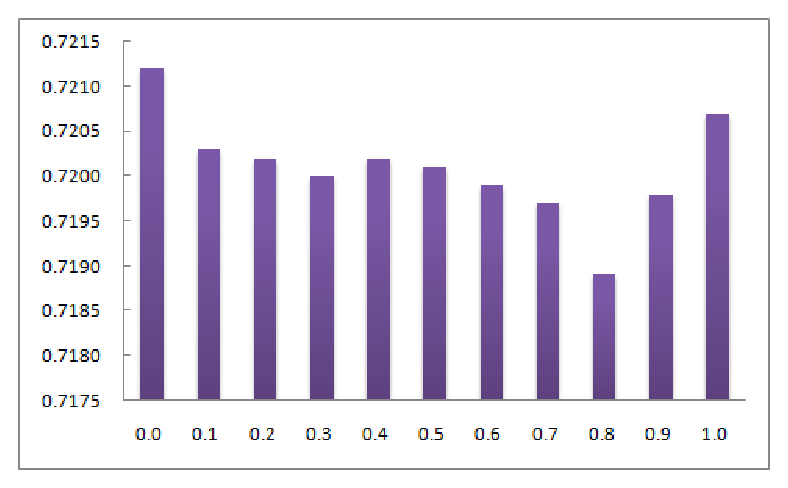
\includegraphics[height=3cm, width=6cm]{XITAMAE.eps}}
			\centerline{(a)MAE}
		\end{minipage}
		\hfill
		\begin{minipage}{0.48\linewidth}
			\centerline{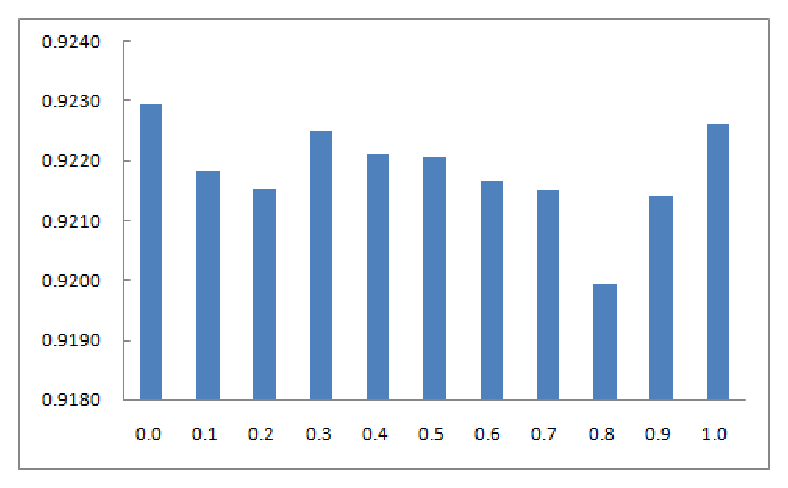
\includegraphics[height=3cm, width=6cm]{XITARSME.eps}}
			\centerline{(b)RMSE}
		\end{minipage}
		\caption{\textbf{Comparisons of different similarity weight of \emph{NAGOP-MF} on MAE and RSME metrics. }}
	\end{figure*}
	We first compare the proposed methods with baseline methods
	and then search the best weight coefficient of similarity.
	Lastly, we evaluate the importance of user attributes in our proposed methods.
	\subsubsection{Method Comparison}
	The prediction errors measured by MAE and RMSE of all methods are reported in Table 6 with best results highlighted in boldface.
	We make four observations from the results.
	
	\begin{table}
		\centering
		\caption{\textbf{MAE and RMSE of all methods, the lower the better.}}
		\begin{tabular}{llll}\hline
			ID & Method & MAE & RMSE \\\hline
			1 &Global Mean &0.9435 &1.1256\\
			2 &User Mean &0.8362 &1.0437\\
			3 &Item Mean &0.8163 &1.0229\\
			4 &RSVD &0.7492 &0.9496\\
			5 &Social MF &0.7372 &0.9304\\
			6 &Biased MF &0.7418 &0.9468\\ \hline
			7 &NA-MF &0.7228 &0.9234\\
			8 &NAG-MF &0.7205 &0.9213\\
			9 &NAGO-MF &0.7193 &0.9204\\
			10 &NAGOP-MF & \textbf{0.7189} &\textbf{0.9199}\\
			11 &NAGOPC-MF &0.7190 &0.9201\\\hline
			12 &AGOP-MF &0.7275 &0.9321\\
			13 &AGOPC-MF &0.7275 &0.9322\\\hline
		\end{tabular}
	\end{table}
	
	
	First, incorporating attributes influence into item rating prediction greatly reduces prediction errors measured
	by both MAE and RMSE. All the proposed methods with attributes influence (i.e., methods 7 - 13) outperform
	all baseline methods (methods 1 - 6). The best prediction accuracy
	is achieved by \emph{NAGOP-MF} which considers neighborhood(\emph{N}), user age(\emph{A}), user gender(\emph{G}), user occupation(\emph{O}) and item
	popularity (\emph{P}). With attribute age influence alone, \emph{NA-MF} outperforms all baselines including state-of-the-art methods \emph{Bias MF} and \emph{Social MF}.
	This result suggests that using user attributes is of great help to item rating prediction.
	Further considering factors like user gender(\emph{G}) and user occupation(\emph{O}) leads to relatively small additional reduction in prediction errors.
	
	Second, without incorporating neighborhood influence, \emph{AGOP-MF}
	performs poorer than most methods with neighborhood influence including \emph{NA-MF}, \emph{NAG-MF}, \emph{NAGO-MF}, \emph{NAGOP-MF} and \emph{NAGOPC-MF}.
	The poorer performance of \emph{AGOP-MF} against \emph{NA-MF} suggests
	that the neighborhood influence is more effective than
	the combination of the three factors (\emph{G}, \emph{O}, and \emph{P}) in item rating
	prediction.
	On the other hand, the effectiveness
	of neighborhood influence is also reflected from the
	better performance of \emph{AGOPC-MF} compared with \emph{NAGOPC-MF}.
	
	Third, incorporating popularity influence, \emph{NAGOP-MF} and \emph{NAGOPC-MF}
	performs better than most methods without popularity influence including \emph{NA-MF}, \emph{NAG-MF}, \emph{NAGO-MF}.
	Such result supports our earlier discussion
	that considering popularity can improve rating prediction accuracy.
	Unnatural, method \emph{NAGOPC-MF} incorporating item popularity(\emph{P}) and item category popularity(\emph{C}) influences performs
	poorer than \emph{NAGOP-MF} only including item popularity influence.
	This may be caused by the noise resulting from using item popularity(\emph{P})
	and item category popularity(\emph{C}) in one prediction model.
	Because item category popularity have certain direct relationship with item popularity.
	
	Last, among the 6 baseline methods, \emph{Social MF}, the
	state-of-the-art methods, perform the best evaluated by both MAE and RMSE.
	While \emph{Global Mean} perform the worst.
	
	\subsubsection{Impact of Different Similarity Weight}
	\begin{figure*}
		\centering
		\begin{minipage}{0.48\linewidth}
			\centerline{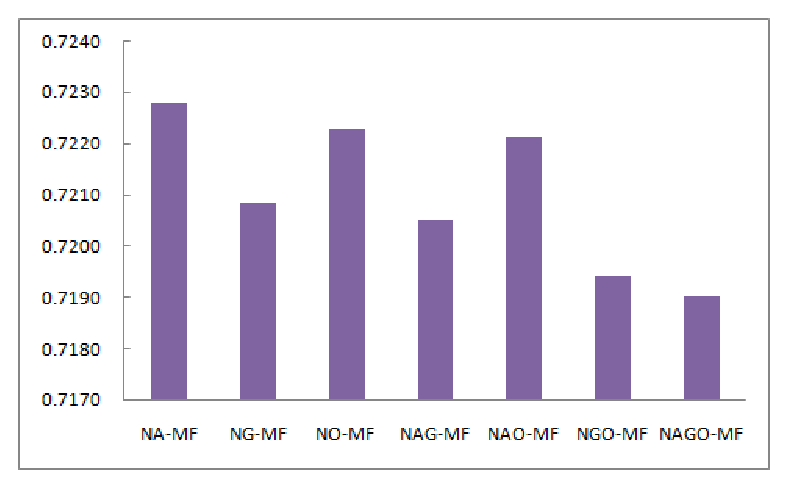
\includegraphics[height=3cm, width=6cm]{MAE.eps}}
			\centerline{(a)MAE}
		\end{minipage}
		\hfill
		\begin{minipage}{0.48\linewidth}
			\centerline{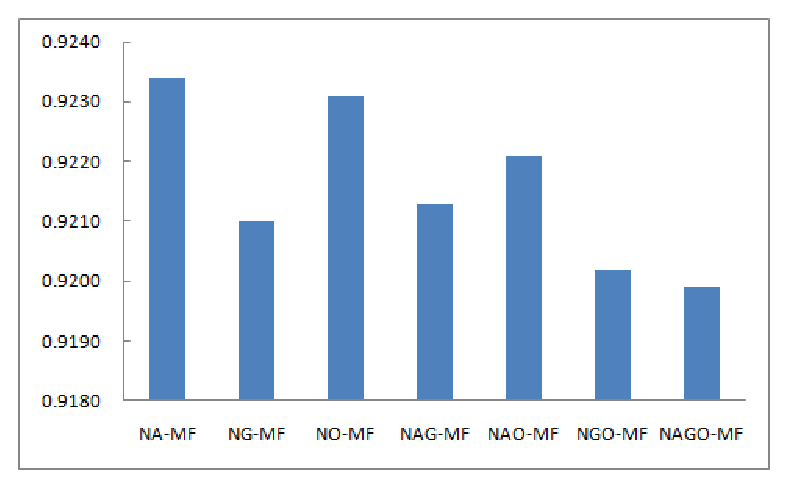
\includegraphics[height=3cm, width=6cm]{RSME.eps}}
			\centerline{(b)RMSE}
		\end{minipage}
		\caption{\textbf{Comparisons of different types of methods on MAE and RSME metrics. }}
	\end{figure*}
	As described in section 4.2, $\gamma$ is a weight coefficient to balance the importance between rating sequence similarity and attribute similarity.
	Bigger $\gamma$ represents attribute similarity is more important and vice versa.
	To explore the impact of $\gamma$ on the rating prediction accuracy,
	we select 11 different $\gamma$ from 0 to 1 to use in the \emph{NAGOP-MF} method.
	The \emph{NAGOP-MF} method is selected as the method for evaluation because it has
	the best performance.
	
	Figures 2(a) and 2(b) respectively plot MAE and RMSE of the
	\emph{NAGOP-MF} method by using different $\gamma$ ranging from 0 to 1.
	From the figure, $\gamma= 0.8$ gives the best prediction accuracy by considering both MAE and RMSE,
	and only using rating similarity($\gamma= 0$) or attribute similarity($\gamma= 1.0$) gets worse results.
	These show that both rating similarity and attribute similarity are help for rating prediction, and
	attribute similarity are more important than rating similarity. This may be caused by that
	users with similar attributes can better reflect the users' close preference than those users with similar rating sequence.
	
	\subsubsection{Analysis of Each Attribute Factor}
	
	Age(\emph{A}), gender(\emph{G}), and occupation(\emph{O}) factor are three main factors for rating prediction in this task. Although the results of \emph{NA-MF},
	\emph{NG-MF}, and \emph{NO-MF} shown in Figure 3 can indicate their effectiveness for the task alone, the contribution
	of each factor to \emph{NAGOP-MF} should also be explored. This is
	because combining multiple latent factors to form a unified model does not mean the results of the new model is the
	performance summarization of each factor.
	
	To better understand the importance of each attribute factor, we also adopt the strategy of combining two factors from user attributes,
	i.e., \emph{NAG-MF}, \emph{NAO-MF} and \emph{NGO-MF}. we keep using neighborhood(\emph{N}) in this section because of user attribute also
	using in neighborhood selection, while item popular(\emph{P}) is moved for the reasons that it has no relationship with user attribute.
	Specifically, we test the strategy of all three user attributes factors using \emph{NAGO-MF}. The results of them are displayed
	in Figure 3. We find \emph{NG-MF} performs clearly better than \emph{NA-MF} and \emph{NO-MF} both in MAE and RSME, which indicates the importance of
	user gender information to the task. The reason may be attributed to the dramatic preference difference between female and male
	as we discussed in section 3.2.
	\emph{NO-MF} achieves better results than \emph{NA-MF}, which reveals age information makes a smaller contribution to \emph{NAGOP-MF} than
	occupation information. This is because the number of user's occupation group is much more than age group, which leads to the
	occupation factors more personalized.
	
	On the other hand, \emph{NGO-MF} performs clearly better than
	the other methods with two attribute factors, which again indicates the top importance of
	gender, occupation take the second and age is the last. Lastly, when all the three attributes are
	combined together(\emph{NAGO-MF}), the performance is further improved, which indicates each
	attribute is good for rating prediction.
	
	\section{CONCLUSION}
	
	In this work we proposed a new, simple, and efficient way
	to incorporate user attributes and item category on ratings prediction in several methods
	commonly used for matrix factorization.
	We firstly analyze the MovieLens dataset and find that a user's rating behavior is certainly
	correlated with his or her attribute type.
	Based on this observation, we model a user with two vectors of latent factors one for its intrinsic characteristics and the other 	for its common characteristics determined by his or her attribute type.
	The experimental results on real dataset have shown that our
	model is effective and outperforms several alternative methods.
	Other factors like user neighbor, item neighbor, item popularity and item category popularity can further improve the rating prediction accuracy.
	Nevertheless, using both item popularity and item category popularity in one method may bring noise and lead to bad results.
	
	
	
	\section{Acknowledgments}
	This research was supported in part by the National Natural
Science Foundation of China under Grant 91124001 and  the Fundamental Research Funds for the Central University, and the Research Funds of Renmin University of China under grant 2015030273. 
	\begin{thebibliography}{[10]}
        \bibitem{SIGIR201301}
		H. Ma. An Experimental Study on Implicit Social Recommendation.
		Proceedings of the 36th international ACM SIGIR conference on Research and development in information retrieval, Pages 73-82, ACM, 2013.

        \bibitem{4-1-1}Y. Koren. Factorization meets the neighborhood: A
		multifaceted collaborative filtering model. In KDD, pages
		426-434. ACM, 2008.

		\bibitem{2-1-1}G. Adomavicius and A. Tuzhilin. Toward the next generation of recommender systems: A survey of the state-of-the-art and possible extensions. TKDE, 17(6):734-749, 2005.
		
        \bibitem{2-1-2}N. Koenigstein, G. Dror, and Y. Koren. Yahoo! music recommendations: Modeling music ratings with temporal dynamics and item taxonomy. In RecSys, pages 165-172. ACM, 2011.
		
       \bibitem{2-1-3}Koen Verstrepen and Bart Goethals. Unifying nearest neighbors collaborative filtering. Proceedings of the 8th ACM Conference on Recommender systems, RecSys'14, Pages 177-184. ACM, 2014.
		
       \bibitem{2-1-4}
		N. Natarajan, D. Shin, and I. S. Dhillon. Which app will you
		use next?: Collaborative filtering with interactional context.
		In RecSys, pages 201-208. ACM, 2013.
		
        \bibitem{cfclass}
		J. S. Breese, D. Heckerman, and C. Kadie, Empirical analysis
		of predictive algorithms for collaborative filtering,  in Proceedings
		of the Fourteenth conference on Uncertainty in artificial intelligence.
		Morgan Kaufmann Publishers Inc., 1998, pp. 43-52.

       \bibitem{uCF}
		R. Jin, J. Y. Chai, and L. Si. An automatic weighting scheme
		for collaborative filtering. In SIGIR, pages 337-344, 2004.
		
		\bibitem{iCF1}
		M. Deshpande and G. Karypis. Item-based top-n
		recommendation algorithms. ACM Trans. Inf. Syst.,
		22(1):143-177, 2004.
		
		\bibitem{iCF2}
		B. Sarwar, G. Karypis, J. Konstan, and J. Riedl. Item-based
		collaborative filtering recommendation algorithms. In WWW,
		pages 285-295. ACM, 2001.

       \bibitem{KDD200801}
		Y. Koren. Factorization Meets the Neighborhood: A Multifaceted Collaborative Filtering Model. Proc. 14th ACM
		SIGKDD Int'l Conf. Knowledge Discovery and Data Mining,ACM Press, 2008, pp. 426-434.
		
       \bibitem{COMPUTER2009}
		Y. Koren, R. Bell, and C. Volinsky. Matrix factorization
		techniques for recommender systems. Computer,42(8):30-37, 2009.

        \bibitem{GeoMF}
		D. Lian, C. Zhao, X. Xie, G. Sun, E. Chen, and Y. Rui. GeoMF: joint geographical modeling and matrix factorization for point-of-interest recommendation
		In Proceedings of KDD' 14, pages 831-840. ACM, 2014.

        \bibitem{SIGIR201401}
		L. Hu, A. Sun and Y. Liu. Your Neighbors Affect Your Ratings: On Geographical
		Neighborhood Influence to Rating Prediction. In Proceedings of the 37th international ACM SIGIR conference on Research \& development in information retrieval,Pages 345-354,ACM,2014.
		
       \bibitem{CIKM201401}
		T. Wang, X. Jin, X. Ding and X. Ye. User Interests Imbalance Exploration in Social
		Recommendation: A Fitness Adaptation.In Proceedings of the 23rd ACM International Conference on Conference on Information and Knowledge Management,Pages 281-290,ACM,2014.

		\bibitem{event1}
		T.-A. N. Pham, X. Li, G. Cong, and Z. Zhang. A general
		graph-based model for recommendation in event-based social
		networks. In ICDE, Seoul, Korea, April 13-17, 2015.
		
		\bibitem{event2}
		W. Zhang and J.Y Wang. A Collective Bayesian Poisson Factorization Model for Cold-start Local Event Recommendation.
		In Proceedings of the 21th ACM SIGKDD International Conference on Knowledge Discovery and Data Mining.
		ACM Press, 2015, Pages 1455-1464. 	
		
		\bibitem{tag}
		W. Feng, J. Wang. We Can Learn Your \#Hashtags: Connecting Tweets to Explicit Topics.In ICDE, Chicago, USA, March 31-April 4, 2014.

		\bibitem{bias}
		
		N. Koenigstein, G. Dror, and Y. Koren. Yahoo! music
		recommendations: Modeling music ratings with temporal
		dynamics and item taxonomy. In RecSys, pages 165-172.
		ACM, 2011.

        \bibitem{popular1}
		P. Cremonesi, Y. Koren, and R. Turrin. Performance of
		recommender algorithms on top-n recommendation tasks. In
		RecSys, pages 39-46. ACM, 2010.
		
		\bibitem{popular2}
		
		H. Steck. Item popularity and recommendation accuracy. In
		RecSys, pages 125-132. ACM, 2011.
				
       \bibitem{4-1-2}Y. Koren. Collaborative filtering with temporal dynamics. In
		KDD, pages 447-456. ACM, 2009.

        \bibitem{4-2-1} H. Ma, D. Zhou, C. Liu, M. R. Lyu, and I. King.
		Recommender systems with social regularization. In
		Proceedings of the fourth ACM international
		conference on Web search and data mining, WSDM
		'11, pages 287-296, Hong Kong, China, 2011.
		
        \bibitem{5-1-1}R. Salakhutdinov and A. Mnih. Probabilistic matrix
		factorization. In Proceedings of Advances in Neural
		Information Processing Systems, NIPS' 07, 2007.
		
%        \bibitem{4-2-2}J. S. Breese, D. Heckerman, and C. Kadie. Empirical analysis of predictive algorithms for collaborative
%		filtering. In Proceedings of the Fourteenth conference on Uncertainty in artificial intelligence, UAI¡¯98, pages 43¨C52, Madison, Wisconsin, %1998.
		
%       \bibitem{PMF}
%		R. Salakhutdinov and A. Mnih. Probabilistic Matrix Factorization, Proc. Advances in Neural Information Processing
%		Systems 20(NIPS 07), ACM Press, 2008, pp. 1257-1264.
		

		
%       \bibitem{CIKM201302}
%		G. Zhao, M. Lee and W. Hse. Community-Based User Recommendation in
%		Uni-Directional Social Networks.In Proceedings of the 22nd ACM international conference on Conference on information and knowledge management,Pages 189-198,ACM,2013.
		

		
%       \bibitem{SIGIR201402}
%		Y. Zhang, G. Lai, M. Zhang, Y. Zhang, Y. Liu and S.  Ma.Explicit Factor Models for Explainable Recommendation
%		based on Phrase-level Sentiment Analysis.
%		In Proceedings of the 37th international ACM SIGIR conference on Research \& development in information retrieval,Pages  83-92 ,ACM,2014.
		
%        \bibitem{ICDM2008}
%		Y. F. Hu, Y. Koren, and C. Volinsky. Collaborative Filteringfor Implicit Feedback Datasets. Proc. IEEE Int'l Conf. Data Mining(ICDM 08), IEEE CS Press, 2008, pp. 263-272.
		
%        \bibitem{CSCW2000}
%		J. Herlocker, J. Konstan, and J. Riedl. Explaining
%		collaborative Filtering recommendations. CSCW, 2000.
		
%       \bibitem{KDD200901}
%		Y. Koren. Collaborative Filtering with Temporal Dynamics. Proc. 15th ACM SIGKDD Int'l Conf. Knowledge Discovery
%		and Data Mining(KDD 09), ACM Press, 2009, Pages 447-455.
		

		
%        \bibitem{WWW2001}
%		B. Sarwar, G. Karypis, J. Konstan, and J. Riedl. Item-based
%		collaborative filtering recommendation algorithms. In WWW,
%		pages 285-295. ACM, 2001.
		
		
\end{thebibliography}
\end{document} 